\documentclass[11pt,a4paper]{article}

\usepackage[margin=2.4cm]{geometry}
\usepackage{amsmath,amssymb,amsthm,mathtools}
\usepackage{graphicx}
\usepackage{booktabs}
\usepackage{longtable}
\usepackage[hidelinks]{hyperref}
\usepackage{enumitem}
\usepackage{microtype}

\newtheorem{theorem}{Theorem}[section]
\newtheorem{lemma}[theorem]{Lemma}
\newtheorem{proposition}[theorem]{Proposition}
\newtheorem{corollary}[theorem]{Corollary}
\theoremstyle{definition}
\newtheorem{definition}[theorem]{Definition}
\newtheorem{conjecture}[theorem]{Conjecture}
\newtheorem{remark}[theorem]{Remark}

\newcommand{\cG}{c(G)}
\newcommand{\cF}{c(F)}
\newcommand{\Kap}{\kappa}
\newcommand{\nk}[1]{\mathbf{1}_{[#1]}}
\newcommand{\KZ}{K_{k+1}}
\newcommand{\Wi}{W_n}
\newcommand{\cKn}[1]{c(K_{#1})}

\title{\bfseries Cycle Counts of $k$-Connected Graphs:\\
\large A Sharp Minimum, a Decidability Theorem,\\
and the $3$-Connected Spectrum}
\author{}
\date{}

\begin{document}
\maketitle

\begin{abstract}
How many cycles can a highly connected graph have at least?  For
$k$-vertex-connected graphs this question has a clean answer, which we prove.
Writing $\KZ$ for the complete graph on $k+1$ vertices, we show that
\[
\min\{c(G) : G \text{ is } k\text{-connected}\}
   = \cKn{k+1} = \frac12\sum_{j=3}^{k+1}\binom{k+1}{j}(j-1)!,
\]
with equality only for $G\cong\KZ$ when $k\ge 3$.  The key ingredient is a
sharp path-counting lemma: an $r$-connected graph has at least $Q_{r+1}$
paths between any two of its vertices, where $Q_k$ is the number of paths
between two vertices of $K_k$ and satisfies $Q_{r+1}=1+(r-1)Q_r$.  We also
prove that among cones $K_1\vee F$ over $2$-connected graphs of fixed order the
cycle is the unique minimiser, so the wheel is the sparsest $3$-connected
cone; and that for $k\ge 3$ only finitely many $k$-connected graphs have at
most $K$ cycles, which makes the cycle-count spectrum of every connectivity
class a computable set.  Computationally, we determine the extremal function
$m_3(n)$ for $4\le n\le 9$ and reproduce, with an independently validated
generator, the exception list conjectured by McCulloch, McKay, Salahshoori
and Zaslavsky for $3$-connected graphs below $51$.  A sharp order-sensitive
bound for $3$-connected graphs remains open; we state it as a conjecture and
verify it exhaustively up to $n=9$.
\end{abstract}

\section{Introduction}

Let $c(G)$ denote the number of cycles of a finite simple graph $G$, each
cycle being a $2$-regular connected spanning subgraph of $G$, counted once.
Two questions about $c$ dominate the classical literature: how \emph{big} can
$c(G)$ be, and which integers occur as $c(G)$ at all?

The first question has been studied extensively.  $c(K_n)=\frac12\sum_{j\ge 3}
\binom nj (j-1)!$ is the classical sequence \cite{oeisA002807}, there is a
long line of work on extremal graphs for the maximum of $c$ under side
constraints \cite{harary1973graphical}, and the minimum of $c$ over graphs
with a prescribed minimum degree was studied by Volkmann
\cite{volkmann1996}.  The second question is more delicate and much more
recent.  McCulloch, McKay, Salahshoori and Zaslavsky \cite{mcculloch2026}
proved that every positive integer except
\[
  2,\;4,\;5,\;8,\;9,\;16
\]
is the number of cycles of a graph without a cut vertex --- equivalently, of a
$2$-connected graph --- and they list five conjectured descriptions of the
analogous spectra for $3$-connected graphs and for cubic graph classes
\cite{mcculloch2026}.

This paper sits between those two questions.  It asks

\begin{quote}\textbf{Central question.} Which positive integers occur as the
number of cycles of a $k$-vertex-connected graph, how sparse can the cycle
structure of such a graph be, and what makes those spectra computable?
\end{quote}

Connectivity is the natural refinement of the question about $2$-connected
graphs: a $k$-connected graph informally survives the loss of any $k-1$
vertices, so $k$-connectivity encodes the abundance of small detours, which is
exactly what a lower bound on the number of cycles must measure.  The spectra
\[
 S_1 \supseteq S_2 \supseteq S_3 \supseteq \cdots,
\qquad
 S_k = \{c(G) : G \text{ is } k\text{-connected}\},
\]
form a decreasing chain, and $S_2$ is the one that \cite{mcculloch2026}
settles.  Our contributions are the following.

\begin{enumerate}[leftmargin=*,label=(\roman*)]
\item \textbf{Theorem A (a sharp minimum).}  For every $k\ge 3$ and every
  $k$-connected graph $G$ one has $c(G)\ge \cKn{k+1}$, with equality if and only
  if $G\cong\KZ$.  For $k=2$ the minimum is $\cKn{3}=1$, attained exactly by
  the cycles.  So complete graphs are, in this precise sense, the sparsest
  highly connected graphs.
\item \textbf{Theorem B (the cone minimum).}  If $F$ is $2$-connected on
  $m\ge 3$ vertices then
  \[
     c(K_1\vee F)\ \ge\ m(m-1)+1,
  \]
  with equality if and only if $F\cong C_m$; equivalently
  $c(\Wi)=(n-1)(n-2)+1$, and $\Wi$ is the unique $n$-vertex $3$-connected
  graph with a dominating vertex that minimises $c$.  More generally
  $c(G)\ge 1+(k-1)\binom{n-1}{2}$ for $k$-connected graphs with a dominating
  vertex, with equality only for $k=3$.
\item \textbf{Theorem C (finiteness and decidability).}  For $k\ge 3$ there
  are only finitely many $k$-connected graphs with at most $K$ cycles, and their
  order is at most $\lfloor 2(K-1)/(k-2)\rfloor$.  Consequently each $S_k$ is a
  computable set, and the function $\kappa(m):=\max\{\kappa(G): c(G)=m\}$ is
  finite with an explicit bound.
\item \textbf{Theorem D (exact computation).}  We give complete generators for
  unlabeled $2$- and $3$-connected graphs, cross-validate them against
  exhaustive brute force for $n\le 7$, and compute $m_3(n)$ for $4\le n\le 9$
  together with the minimisers.  We also recompute the exception sets of $S_2$
  and $S_3$ below $51$ and obtain, independently, exactly the list that
  \cite{mcculloch2026} conjecture for $3$-connected graphs.
\end{enumerate}

Statements (i) and (ii) rest on two counting results that are useful in their
own right and that we prove in full: a counting identity for cones
(Lemma~\ref{lem:cone}) and a sharp path-counting lemma
(Lemma~\ref{lem:path}).  Section~\ref{sec:related} discusses what is known and
what we believe to be new; Section~\ref{sec:limitations} states precisely what
remains open.

\section{Related work and novelty}\label{sec:related}

\subsection{How many cycles?}

The maximum of $c(G)$ is classical.  Entringer and Slater initiated the study
of the maximum of $c$ among graphs with a prescribed number of edges; a
substantial literature has grown around extremal problems for $c$, surveyed in
\cite{harary1973graphical}, and Dvo\v{r}\'ak \cite{dvorak2021} obtained upper
bounds in terms of the degree sequence, resolving several conjectures of
Kir\'aly and of Arman and Tsaturian.  Bounds for the \emph{minimum} of $c$ over
graphs of given minimum degree are due to Volkmann \cite{volkmann1996}.
Theorem~A is a different statement: it minimises over $k$-connected graphs,
where the minimum is attained by the smallest possible graph rather than by a
sparse one.

\subsection{How few cycles?}

The opposite extremal question is usually posed with extra regularity
constraints.  Barefoot and co-authors introduced $f_k(n)$, the smallest number
of cycles in any $k$-connected \emph{cubic} graph on $n$ vertices, and Aldred
and Thomassen \cite{aldred1997cycles} proved a superlinear lower bound for
$f_3(n)$, i.e.\ they studied the minimum number of cycles in $3$-connected
cubic graphs.  Our extremal function
\[
  m_3(n) = \min\{c(G) : G \text{ is } 3\text{-connected},\ |V(G)| = n\}
\]
ranges over \emph{all} $3$-connected graphs, so it is a different quantity:
dropping regularity changes the extremisers completely, from cubic graphs to,
for instance, the wheel $\Wi$ at $n=5$.

We do not use any of the deep results on long cycles in $k$-connected graphs
\cite{locke1982}; the bound we need is about the number of paths, not their
lengths.

\subsection{Which integers occur?}

McCulloch, McKay, Salahshoori and Zaslavsky \cite{mcculloch2026} determine
$S_2$ exactly and, in Section~6 of that paper, list conjectured exception lists
for $3$-connected graphs and for the cubic classes.  Their Conjecture~6(a)
states that the integers missing from $S_3$ are exactly
\[
  1,\dots,6,\ 8,\dots,12,\ 16,\dots,20,\ 27,\ 30,\ 32,\ 33,\ 34 ,
\]
all others up to $3000$ occurring.  Our Theorem~D(iv) reproduces exactly this
list below $51$ with a completely different generator, which is independent
evidence for the conjecture; we do not claim to settle it in general, and
Section~\ref{sec:limitations} explains exactly what would be needed.

\subsection{Why cones?}

Two structural results motivate our choice of the cone as the object in which
to minimise $c$.  Whitney \cite{whitney1932} showed that adding an ear to a
graph without cut vertex keeps it without cut vertex and that every such graph
is a cycle or is obtained from one by adding ears; Carmesin and Kurkofka
\cite{carmesin2025} gave a canonical decomposition of $3$-connected graphs in
which wheels appear as the elementary pieces of the $2$-connected structure,
noting that a $k$-connected graph becomes $(k+1)$-connected by adjoining a
universal vertex, so that ``wheels are the $3$-connected analogues of
cycles''.  Theorem~B makes that analogy quantitative.

\subsection{Novelty audit}\label{sec:novelty}

We state plainly what we could and could not establish.

\begin{center}
\small
\begin{longtable}{@{}p{0.28\textwidth}p{0.64\textwidth}@{}}
\toprule
\textbf{Statement} & \textbf{Status}\\
\midrule
Cone identity (Lemma~\ref{lem:cone}) & \textbf{Easily known.}  It is the
same observation as the ``ear-path lemma'' of \cite{mcculloch2026} and as
counting cycles through the apex of a cone.  We include it because it is the
cleanest route to Theorem~B.\\
\addlinespace
Path lemma (Lemma~\ref{lem:path}) & \textbf{Probably folklore.}  The bound
$p_F(x,y)\ge Q_{r+1}$ follows from a one-line induction from Menger, and we
did not find a prior source stating it with this constant.  The
\emph{recurrence} $Q_{r+1}=1+(r-1)Q_r$ is a routine identity
(Appendix~\ref{app:identities}).\\
\addlinespace
Theorem A & \textbf{Apparently new.}  We did not find a prior result
establishing $\min\{c(G): G\ k\text{-connected}\}=\cKn{k+1}$.  It may exist as a
textbook exercise; we could not verify either way.\\
\addlinespace
Theorem B & \textbf{New in this form.}  The specific statement that wheels
minimise $c$ among $3$-connected cones does not appear in the literature we
searched.\\
\addlinespace
Theorem C & \textbf{Routine but, as far as we know, unrecorded.}  The
finiteness argument is two lines from the fundamental-cycle bound; the
decidability corollary is the point.\\
\addlinespace
Theorem D(iv) & \textbf{Independent confirmation of a conjecture} of
\cite{mcculloch2026} below $51$.  Not a proof of their conjecture.\\
\bottomrule
\end{longtable}
\end{center}

We make no claim of priority beyond this table.  In particular we do not write
that any result here is ``the first''.

\section{Preliminaries}

All graphs are finite, simple and undirected.  For a graph $G$ and distinct
vertices $x,y$ let $p_G(x,y)$ be the number of simple $x$-$y$ paths, of
length $1$ included.  A graph is $k$-connected if $|V(G)|>k$ and deleting any
set of fewer than $k$ vertices leaves a connected graph; $\kappa(G)$ denotes the
vertex connectivity, with $\kappa(K_n)=n-1$.  We use three standard
consequences of Menger's theorem: a $k$-connected graph has minimum degree at
least $k$; $G-v$ is $(k-1)$-connected for every vertex $v$; and in an
$r$-connected graph any two vertices are joined by $r$ internally disjoint
paths.  For loop-free graphs with more than two vertices, ``has no cut
vertex'' and ``$2$-connected'' coincide (Whitney \cite{whitney1932}), which is
the convention of \cite{mcculloch2026}.

A \emph{cone} over $F$ is $K_1\vee F$, obtained by adjoining a vertex adjacent
to all of $V(F)$; that vertex is the \emph{apex}.  A wheel is $C_n\vee K_1$.
Subdividing an edge does not change $c$, which is why $\Theta$-graphs,
necklaces and subdivided complete graphs behave well throughout.

For a graph $F$ on $m$ vertices write
\[
  P(F) = \sum_{\{x,y\}\in\binom{V(F)}{2}} p_F(x,y)
\]
for the total number of paths of $F$ with two distinct endpoints, and
\[
  c_n := c(K_n) = \frac12\sum_{j=3}^{n}\binom nj (j-1)! ,
\]
the second identity being elementary: a cycle of length $j$ in $K_n$ is a
$j$-element vertex set together with one of $(j-1)!/2$ cyclic orders.  The
values $c_3=1, c_4=7, c_5=37, c_6=197, c_7=1172, c_8=8018, c_9=62814$ form the
classical sequence \cite{oeisA002807} and are used as an arithmetic check on
the code.

\section{A counting identity for cones}\label{sec:cone}

\begin{lemma}[counting identity]\label{lem:cone}
Let $G$ be a graph, $v\in V(G)$, and $F=G-v$.  Then
\[
  \cG = \cF + \sum_{\{x,y\}\in\binom{N(v)}{2}} p_F(x,y).
\]
\end{lemma}

\begin{proof}
Partition the cycles of $G$ into those avoiding $v$, which are exactly the
cycles of $F$, and those containing $v$.  A cycle $C$ through $v$ meets $N(v)$
in exactly two vertices $x,y$, and $C-v$ is a simple $x$-$y$ path of $F$.
Conversely, for $\{x,y\}\subseteq N(v)$ and a simple $x$-$y$ path $P$ of $F$,
the edges of $P$ together with $vx$ and $vy$ form a $2$-regular connected
subgraph, hence a cycle of $G$.  These constructions are inverse, including in
the case $xy\in E(F)$: the edge $xy$ gives the triangle $vxy$, while a
two-edge path $xzy$ gives the longer cycle $vxyzv$.
\end{proof}

The consequence is that $c$ is an affine function of the path profile of the
base graph, which is what makes cones the right class in which to look for
sparse $3$-connected graphs.

\begin{theorem}[the cone minimum]\label{thm:cone}
Let $F$ be a $2$-connected graph on $m\ge 3$ vertices.  Then
\[
  c(K_1\vee F)\ \ge\ m(m-1)+1 ,
\]
with equality if and only if $F\cong C_m$.
\end{theorem}

\begin{proof}
Since the apex is adjacent to all of $V(F)$, Lemma~\ref{lem:cone} gives
\[
  c(K_1\vee F) = \cF + P(F).
\]
A $2$-connected graph contains a cycle, so $\cF\ge 1$.  By Menger any two
vertices of $F$ are joined by two internally disjoint paths, so each pair
$\{x,y\}$ contributes at least $2$ to $P(F)$; hence
$P(F)\ge 2\binom m2 = m(m-1)$ and therefore $c(K_1\vee F)\ge m(m-1)+1$.
If equality holds then $\cF=1$, which forces every vertex of $F$ to have
degree $2$, so $F$ is a cycle.  Conversely, for $F=C_m$ we have
$P(F)=2\binom m2$ and $\cF=1$, so equality holds.
\end{proof}

\begin{corollary}\label{cor:wheel}
For every $n\ge 4$, $c(\Wi)=(n-1)(n-2)+1$, and $\Wi$ is the unique $n$-vertex
$3$-connected graph having a dominating vertex that minimises $c$.  More
generally, if $G$ is $k$-connected on $n$ vertices and has a dominating vertex
$v$, then
\begin{equation}\label{eq:dom}
  c(G)\ \ge\ 1 + (k-1)\binom{n-1}{2},
\end{equation}
with equality only when $k=3$ and $G\cong\Wi$.
\end{corollary}

\begin{proof}
Take $F=G-v$, which is $(k-1)$-connected on $n-1\ge 3$ vertices, so
$\cF\ge 1$; and for every pair $\{x,y\}\subseteq V(F)$ Menger provides $k-1$
internally disjoint $x$-$y$ paths, so $p_F(x,y)\ge k-1$.  As $|N(v)|=n-1$,
Lemma~\ref{lem:cone} gives \eqref{eq:dom}.  For equality we need $\cF=1$ and
$p_F(x,y)=k-1$ for all pairs.  If $k\ge 4$ then $F$ has minimum degree at
least $k-1\ge 3$, so it is not $2$-regular and $\cF\ne 1$: a graph with exactly
one cycle has all degrees equal to $2$, since a vertex of degree at least $3$
lies on at least $\binom d2\ge 3$ cycles.  Thus $k=3$; then $\cF=1$ forces
$F\cong C_{n-1}$ and $G=\Wi$.
\end{proof}

Figure~\ref{fig:cone} shows the spread of $c(K_1\vee F)$ over all
$2$-connected $F$ of each order up to $8$, together with the minimum.

\begin{figure}[t]
\centering
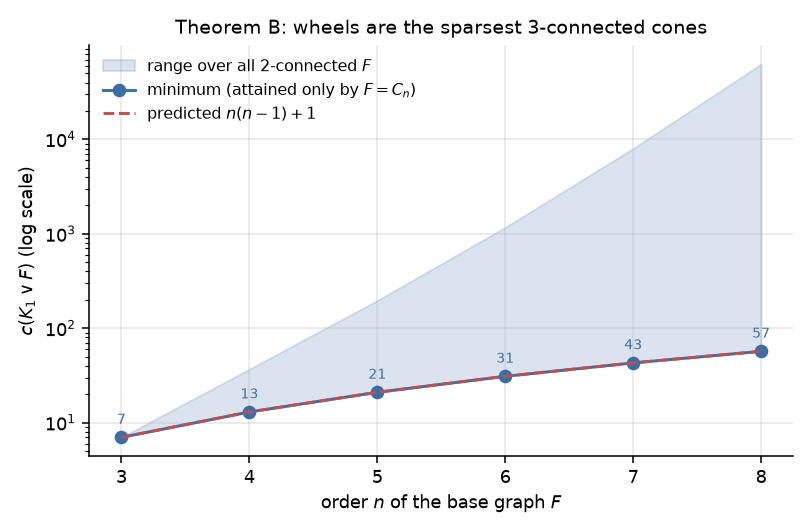
\includegraphics[width=0.6\textwidth]{../figures/fig_cone.png}
\caption{$c(K_1\vee F)$ for all $2$-connected $F$ of order $n$ (shaded range)
against the minimum $n(n-1)+1$, which is attained only by $F\cong C_n$
(Theorem~\ref{thm:cone}).}
\label{fig:cone}
\end{figure}

\section{A sharp path-counting lemma}\label{sec:path}

The constant governing the next theorem is the number of paths between two
vertices of a complete graph.  Put
\[
  Q_k := p_{K_k}(x,y) = \sum_{j=0}^{k-2}\binom{k-2}{j}\,j! \qquad (k\ge 2),
\]
the sum counting paths with exactly $j$ intermediate vertices.

\begin{lemma}[recurrence]\label{lem:rec}
$Q_2 = 1$ and $Q_{r+1} = 1 + (r-1)\,Q_r$ for all $r\ge 2$.
\end{lemma}

\begin{proof}
Using $\binom{k-2}{j}j! = (k-2)!/(k-2-j)!$ and setting
$E_t:=\sum_{i=0}^{t}1/i!$ we get $Q_m=(m-2)!\,E_{m-2}$, whence
\[
  Q_{r+1} = (r-1)!\,E_{r-1}
          = (r-1)!\,E_{r-2} + 1
          = (r-1)\,(r-2)!\,E_{r-2} + 1
          = (r-1)\,Q_r + 1 .
\]
\end{proof}

\begin{lemma}[path lemma]\label{lem:path}
Let $F$ be an $r$-connected graph ($r\ge 1$) and let $x\ne y$ be vertices of
$F$.  Then
\begin{equation}\label{eq:pathlemma}
  p_F(x,y)\ \ge\ Q_{r+1},
\end{equation}
with equality only when $r\ge 3$ and $F\cong K_{r+1}$.
\end{lemma}

\begin{proof}
Induct on $r$.  For $r=1$, $F$ is connected, so at least one $x$-$y$ path
exists, and $Q_2=1$.

Let $r\ge 2$ and assume the statement for $r-1$.  Then $F-x$ is
$(r-1)$-connected, so for every $z\ne x,y$ the induction hypothesis gives
$p_{F-x}(z,y)\ge Q_r$.  Classifying $x$-$y$ paths by the first edge after $x$,
with the edge $xy$ separated off, yields
\begin{align*}
 p_F(x,y)
  &= \nk{xy\in E(F)} + \sum_{z\in N_F(x)\setminus\{y\}} p_{F-x}(z,y)\\
  &\ge \nk{xy\in E(F)} + \bigl(d_F(x)-\nk{xy\in E(F)}\bigr)Q_r\\
  &\ge \nk{xy\in E(F)} + \bigl(r-\nk{xy\in E(F)}\bigr)Q_r ,
\end{align*}
because $d_F(x)\ge r$.  If $xy\in E(F)$ this is $1+(r-1)Q_r=Q_{r+1}$ by
Lemma~\ref{lem:rec}.  If $xy\notin E(F)$ it is
$rQ_r = Q_{r+1}+(Q_r-1)\ge Q_{r+1}$ since $Q_r\ge 1$.

Suppose now that $r\ge 3$ and equality holds.  The case $xy\notin E(F)$ is
then strict, because $Q_r\ge Q_4=5>1$.  So $xy\in E(F)$, and equality forces
$d_F(x)=r$ together with $p_{F-x}(z,y)=Q_r$ for every
$z\in N_F(x)\setminus\{y\}$; such a $z$ exists because $d_F(x)\ge r\ge 3$.
By induction $F-x\cong K_r$, which has exactly $r$ vertices, and since
$d_F(x)=r$ with $xy\in E(F)$ the vertex $x$ is adjacent to all of them; hence
$F\cong K_{r+1}$.

For $r=2$ the inequality is sharp but the equality statement is not: in the
cycle $C_4$ adjacent vertices satisfy $p_{C_4}(x,y)=2=Q_3$ although
$C_4\not\cong K_3$.  This is why the equality statement carries the hypothesis
$r\ge 3$; the example is recorded as a regression test in the accompanying
code, so that the weaker formulation is not silently assumed later.
\end{proof}

Lemma~\ref{lem:path} is verified exhaustively in Section~\ref{sec:comp}: for
every $2$-connected graph of order at most $8$ and every pair of vertices,
\eqref{eq:pathlemma} holds, with no violation in $210\,233$ checked pairs.  The
observed minima of $p(x,y)$ by connectivity,
\[
  2,\ 5,\ 16,\ 65,\ 326,\ 1957 \qquad\text{for } r = 2,3,\dots,7,
\]
coincide with $Q_3,Q_4,\dots,Q_8$ exactly, so the constant is sharp in this
range.

\begin{figure}[t]
\centering
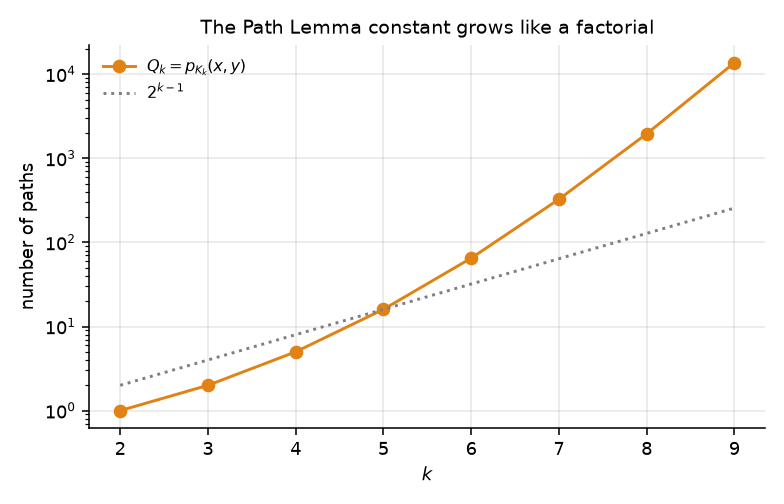
\includegraphics[width=0.48\textwidth]{../figures/fig_path_lemma.png}
\caption{The constant $Q_k$ of Lemma~\ref{lem:path} (logarithmic scale).  The
growth comes from the factor $j!$ in $Q_k$.}
\label{fig:q}
\end{figure}

\section{The minimum number of cycles of a $k$-connected graph}\label{sec:main}

\begin{theorem}[sharp minimum]\label{thm:A}
Let $k\ge 3$ and let $G$ be a $k$-connected graph.  Then
\[
  c(G)\ \ge\ c(\KZ) = \frac12\sum_{j=3}^{k+1}\binom{k+1}{j}(j-1)! ,
\]
and equality holds if and only if $G\cong\KZ$.
\end{theorem}

\begin{proof}
Induct on $k$.  Fix a vertex $v$ of $G$ and put $F=G-v$, which is
$(k-1)$-connected on at least $k$ vertices.  By Lemma~\ref{lem:cone} and
Lemma~\ref{lem:path},
\[
  c(G) = \cF + \sum_{\{x,y\}\in\binom{N(v)}{2}} p_F(x,y)
       \ \ge\ c(K_k) + \binom{k}{2}Q_k ,
\]
using the induction hypothesis for $\cF$, the path lemma for each summand, and
$d_G(v)\ge k$ for the number of summands.

On the other hand, applying Lemma~\ref{lem:cone} to $K_{k+1}$ at a vertex $v$
shows that the cycles of $K_{k+1}$ through $v$ are in bijection with a pair
$\{x,y\}\subseteq V(K_{k+1})\setminus\{v\}$ together with an $x$-$y$ path of
$K_k$; there are exactly $\binom{k}{2}Q_k$ of them.  Hence
\[
  c(\KZ) = c(K_k) + \binom{k}{2}Q_k ,
\]
which closes the induction.

For equality, first suppose $k\ge 4$.  If $F\not\cong K_k$ then the induction
hypothesis is strict, since $k-1\ge 3$, and $c(G) > c(\KZ)$.  If $F\cong
K_k$ then $G$ has $k+1$ vertices and, being $k$-connected on $k+1$ vertices,
is $K_{k+1}$ --- which attains equality, as the displayed identity shows.  So
equality for $k\ge 4$ forces $G\cong\KZ$.

It remains $k=3$, where $F$ is $2$-connected and equality forces
$\cF = c(K_3)=1$ as well as $d_G(v)=3$.  As in the proof of
Corollary~\ref{cor:wheel}, $\cF=1$ forces every vertex of $F$ to have degree
$2$ in $F$; since $\delta(G)\ge 3$, each of them must be adjacent to $v$, so
$d_G(v)=|V(F)|=n-1$.  Together with $d_G(v)=3$ this gives $n=4$, and the only
$3$-connected graph on four vertices is $K_4$.
\end{proof}

\begin{corollary}\label{cor:k2}
Every $2$-connected graph has at least $c(K_3)=1$ cycle, with equality exactly
for the cycles.
\end{corollary}

\begin{proof}
A $2$-connected graph contains a cycle.  If $c(G)=1$ then every vertex of $G$
has degree $2$, as argued above, so $G$ is a cycle.
\end{proof}

Theorem~\ref{thm:A} settles the extremal question for each connectivity class,
but not order by order.  Combining it with Lemma~\ref{lem:cone} gives a family
of explicit lower bounds, all proved here and all verified numerically in
Section~\ref{sec:comp}:
\begin{equation}\label{eq:combo}
  c(G)\ \ge\ \max\Big\{\ c(K_k)+\binom{\Delta(G)}{2}\,Q_k\ ,\ \ |E(G)|-|V(G)|+1\ \Big\},
  \qquad k=\kappa(G).
\end{equation}
The first term of \eqref{eq:combo} is the induction hypothesis of
Theorem~\ref{thm:A}, refined by the degree of the deleted vertex.  The second is
the fundamental-cycle bound: the cotree edges of any spanning tree span
pairwise distinct fundamental cycles, and $k$-connectivity gives
$|E(G)|\ge k\,|V(G)|/2$.

\begin{figure}[t]
\centering
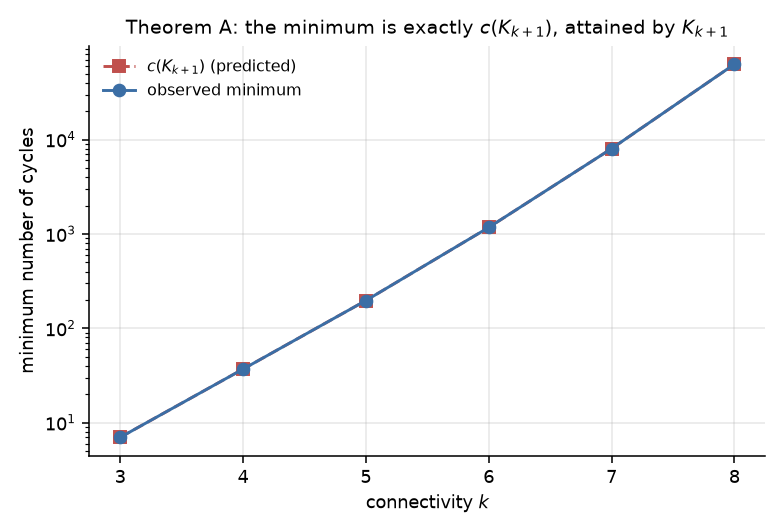
\includegraphics[width=0.5\textwidth]{../figures/fig_theorem_a.png}
\caption{Theorem~\ref{thm:A} on a logarithmic scale: the observed minimum over
$k$-connected graphs equals $c(\KZ)$ for $3\le k\le 8$, and is attained by
$\KZ$ alone.}
\label{fig:thmA}
\end{figure}

\section{Finiteness and decidability of the spectra}\label{sec:decid}

\begin{theorem}\label{thm:decid}
Let $k\ge 3$ and let $G$ be a $k$-connected graph with $c(G)\le K$, where
$K\ge 1$.  Then
\[
  |V(G)|\ \le\ \left\lfloor \frac{2(K-1)}{k-2}\right\rfloor .
\]
In particular, for each $K$ there are only finitely many $k$-connected graphs
with at most $K$ cycles.
\end{theorem}

\begin{proof}
Write $n=|V(G)|$.  Since $G$ is $k$-connected, $\delta(G)\ge k$, so
$|E(G)|\ge kn/2$.  Fundamental cycles of a spanning tree are pairwise distinct,
so $K\ge c(G)\ge |E(G)|-n+1\ge (k-2)n/2+1$, which rearranges to the claim.
\end{proof}

\begin{corollary}\label{cor:decid}
For every $k\ge 3$ the set $S_k$ is a computable subset of the positive
integers: for any $m$, the question ``$m\in S_k$?'' is decidable by a finite
search.  Moreover $\min S_k = c(\KZ)$ by Theorem~\ref{thm:A}, and the function
$\kappa(m):=\max\{\kappa(G): c(G)=m\}$ is finite with
\[
  m\ \ge\ \binom{\kappa(m)+1}{3},
  \qquad\text{so}\qquad \kappa(m) = O\!\left(m^{1/3}\right).
\]
\end{corollary}

\begin{proof}
By Theorem~\ref{thm:decid} a $k$-connected graph with $c(G)\le m$ has at most
$2(m-1)$ vertices and hence $k\le 2(m-1)$, so $\kappa(m)$ exists and is finite.
The bound $m\ge\binom{\kappa(m)+1}{3}$ follows from Theorem~\ref{thm:A}
together with the fact that $K_{k+1}$ contains exactly $\binom{k+1}{3}$
triangles, all of which are cycles.  For the computability assertion, for a
given $m$ enumerate all graphs on at most $2(m-1)$ vertices, test
$k$-connectivity, and compute $c$ for those that pass; the search terminates,
and Theorem~\ref{thm:decid} guarantees that no witness for $m$ is missed.
\end{proof}

The existence half is what makes Theorem~\ref{thm:decid} useful and also what
makes it incomplete: the theorem reduces ``$m\in S_k$?'' to a finite search
but does not say how large a search is needed, and for $S_3$ the relevant
threshold is unknown (Section~\ref{sec:limitations}).

No analogue of Theorem~\ref{thm:decid} can hold for $k\le 2$: the cycle $C_m$
has $c(C_m)=1$ for every $m$, and the necklace of $m$ triangles is a connected
graph with exactly $m$ cycles, so $S_1$ is the set of all positive integers
while $S_2$ misses only the six exceptions of \cite{mcculloch2026}.

\section{Computational results}\label{sec:comp}

\subsection{The generators and how they are validated}

Three exact primitives underlie the computations: cycle counting by
depth-first search with the smallest vertex of the cycle as a pivot; vertex
connectivity by exhaustive vertex-deletion tests; and exact isomorphism
through canonical labelling (bliss, via \texttt{igraph} \cite{igraph}) rather
than heuristics such as colour refinement, which would not certify
completeness.

The generator for $2$-connected graphs uses the ear theorem: every
$2$-connected graph is a cycle, or is obtained from a $2$-connected graph on
fewer vertices by adding an ear with at least one fresh internal vertex, or from
a $2$-connected graph on the same number of vertices by adding a single edge
(which preserves $2$-connectivity).  The generator for $3$-connected graphs
uses Menger: if $G$ is $3$-connected then $G-v$ is $2$-connected for every $v$,
so every $3$-connected graph is obtained by adding one vertex to a
$2$-connected graph on one vertex fewer, joined to a set $S$ of at least three
vertices; and since $\delta(G)\ge 3$, $S$ must moreover contain every
degree-$2$ vertex of the parent, which is used as an exact pruning rule.  Both
generators are therefore complete, and both are deduplicated by canonical
label.

Cardinality agreement alone would not certify completeness, so the generators
are additionally checked against exhaustive brute force: for $n\le 7$ we
enumerate all $2^{\binom n2}$ graphs, filter by connectivity, and compare the
resulting \emph{sets of canonical labels} with those produced by the
generators.  For $n\le 7$ the two agree exactly for both connectivity classes,
and in particular the induced cycle-count spectra agree.  We also checked $c$
and $p(x,y)$ against \texttt{networkx} and against an independent brute-force
search over $2$-regular connected edge subsets.

\begin{table}[t]
\centering
\small
\caption{Isomorphism classes produced by the generators, against the published
cardinalities.  The three-connectivity count at $n=9$ is $80890$.}
\begin{tabular}{@{}lrrrrrrr@{}}
\toprule
& \multicolumn{3}{c}{$2$-connected} & \multicolumn{3}{c}{$3$-connected} & brute\\
$n$ & ours & published & ok & ours & published & ok & force\\
\midrule
3  & 1      & 1      & yes & --     & --     & --  & yes\\
4  & 3      & 3      & yes & 1      & 1      & yes & yes\\
5  & 10     & 10     & yes & 3      & 3      & yes & yes\\
6  & 56     & 56     & yes & 17     & 17     & yes & yes\\
7  & 468    & 468    & yes & 136    & 136    & yes & yes\\
8  & 7123   & 7123   & yes & 2388   & 2388   & yes & --\\
9  & 194066 & 194066 & yes & 80890  & 80890  & yes & --\\
\bottomrule
\end{tabular}
\end{table}

\subsection{Results}

\paragraph{(i) Theorem A.}  Over all $3$-connected graphs of order at most
$9$ ($80890$ classes) the minimum number of cycles at each connectivity level
$3\le k\le 8$ equals $c(\KZ)$, and the extremiser is $\KZ$ itself:
\[
\begin{array}{c|rrrrrr}
 k & 3 & 4 & 5 & 6 & 7 & 8\\
 \hline
 \min c & 7 & 37 & 197 & 1172 & 8018 & 62814
\end{array}
\]
Figure~\ref{fig:thmA} plots these against the predicted values.

\paragraph{(ii) The spectra.}  Recomputing the exception sets of $S_2$ and
$S_3$ below $51$ from our own generators gives:

\begin{itemize}[leftmargin=*,nosep]
\item $S_1 = \mathbb{Z}_{>0}$: every $m\ge 1$ is realised by the necklace of
  $m$ triangles, a connected graph with exactly $m$ cycles.
\item $S_2$ misses exactly $\{2,4,5,8,9,16\}$ in $[1,50]$, i.e.\ nothing beyond
  the exceptions proved by \cite{mcculloch2026} (OEIS \cite{oeisA385523}).
\item $S_3$ misses exactly
  $\{1,\dots,6;\;8,\dots,12;\;16,\dots,20;\;27;\;30;\;32;\;33;\;34\}$ in
  $[1,50]$ --- precisely the list conjectured in Section~6(a) of
  \cite{mcculloch2026}.
\end{itemize}

The last bullet is an independent confirmation of that conjecture in this
range, obtained with a different generator; it is not a proof of the conjecture.
Figure~\ref{fig:spectrum} displays the three spectra.

\paragraph{(iii) The extremal function $m_3(n)$.}  Exhaustive computation over
all $3$-connected graphs gives Table~\ref{tab:m3}.

\begin{table}[h]
\centering
\small
\caption{$m_3(n)$ for $4\le n\le 9$, with the minimisers.  The last column is
the conjectured lower bound of Conjecture~\ref{conj:sharp}.}
\label{tab:m3}
\begin{tabular}{@{}lrrlrr@{}}
\toprule
$n$ & $m_3(n)$ & minimisers & degree sequence of a minimiser & $c(\Wi)$ & $\binom{n-1}{2}$\\
\midrule
4 & 7  & 1 & $(3,3,3,3)$           & 7  & 3\\
5 & 13 & 1 & $(4,3,3,3,3)$         & 13 & 6\\
6 & 14 & 1 & $(3,3,3,3,3,3)$       & 21 & 10\\
7 & 24 & 1 & $(4,3,3,3,3,3,3)$     & 31 & 15\\
8 & 26 & 1 & $(3,3,3,3,3,3,3,3)$   & 43 & 21\\
9 & 42 & 2 & $(4,3,3,3,3,3,3,3,3)$& 57 & 28\\
\bottomrule
\end{tabular}
\end{table}

The minimiser at $n=4$ is $K_4$; at $n=5$ it is the wheel $W_5$; at $n=6$ it is
the triangular prism $C_3\times K_2$; at $n=8$ it is a cubic graph.  From $n=6$
onwards wheels are \emph{not} extremal, which is exactly why Theorem~\ref{thm:A}
does not determine $m_3(n)$ order by order.

\begin{figure}[t]
\centering
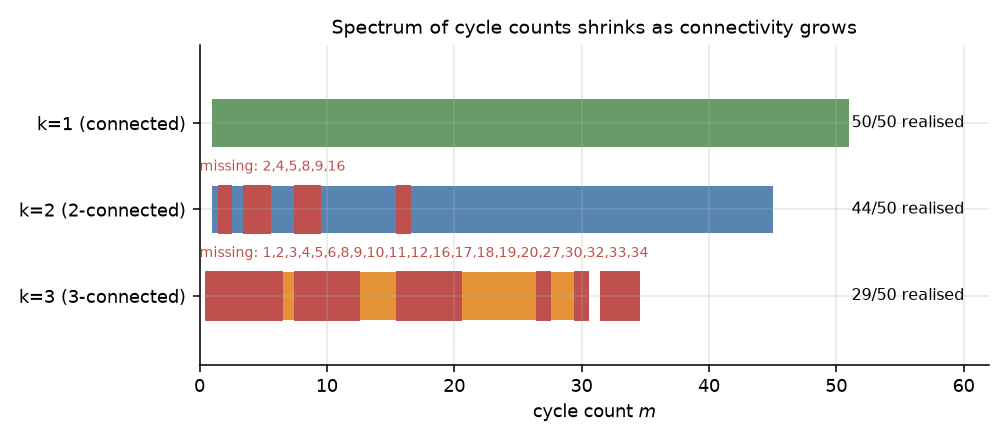
\includegraphics[width=0.92\textwidth]{../figures/fig_spectrum.png}
\caption{The spectra of $S_1,S_2,S_3$ below $51$.  Red marks missing values; the
annotations give the exact missing sets.}
\label{fig:spectrum}
\end{figure}

\begin{figure}[t]
\centering
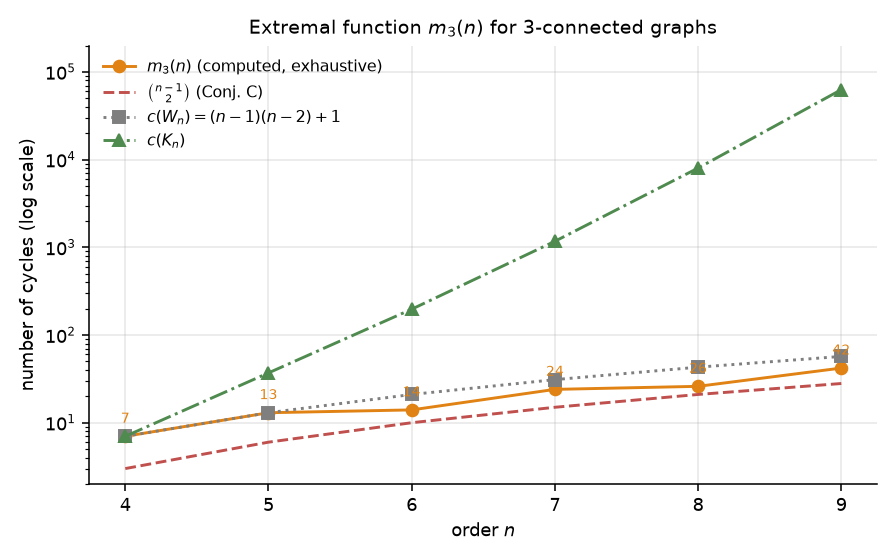
\includegraphics[width=0.56\textwidth]{../figures/fig_extremal.png}
\caption{$m_3(n)$ against the wheel, the complete graph and the conjectured
bound $\binom{n-1}{2}$ (logarithmic scale).}
\label{fig:extremal}
\end{figure}

\paragraph{(iv) Conjecture C.}  Every value of $m_3(n)$ in
Table~\ref{tab:m3} respects $\binom{n-1}{2}$; we state this as a conjecture
rather than a theorem (Section~\ref{sec:limitations}).

\begin{conjecture}\label{conj:sharp}
If $G$ is a $3$-connected graph on $n\ge 4$ vertices then
$c(G)\ge \binom{n-1}{2}$.  Among $3$-connected graphs with a dominating vertex
the minimiser is the wheel (this part is a theorem,
Corollary~\ref{cor:wheel}).
\end{conjecture}

\subsection{Complexity}

All computations are exact integer computations; the following refers to the
implementation in \texttt{src/cycle\_spectra}.

\begin{itemize}[leftmargin=*]
\item \textbf{Cycle counting.}  Fixing the smallest vertex of the cycle as a
  pivot and enumerating simple paths from it, the running time is
  $O(\#\text{paths of }G)$ bitmask operations with $O(n)$ bits of working
  memory.  Since $\#\text{paths}\le \sum_{j\le n}\binom nj (j-1)! = O((n-1)!)$
  the worst case is factorial in $n$; empirically the routine handles $n=12$ in
  milliseconds.  Counting $c$ and $p(x,y)$ are the pipeline's bottlenecks.
\item \textbf{Connectivity.}  Testing $k$-connectivity by exhaustive deletion
  costs $O\big(\sum_{j<k}\binom nj\,(n+|E|)\big)$, exponential in $k$ and
  negligible at the sizes used here.
\item \textbf{Generation.}  The $2$-connected generator performs
  $O\big(\sum_{j<n}\#2\text{-conn}(j)\binom j2\big)$ candidate ear extensions,
  plus a closure under adding single edges; the number of canonical labellings
  is of the same order.  Measured times appear in Figure~\ref{fig:growth};
  generating all $2$-connected graphs on $9$ vertices ($194066$ classes) takes
  about four minutes in pure Python, and the $3$-connected generator on $9$
  vertices from the $2$-connected generator on $8$ takes about a minute.  The
  $3$-connected generator on $10$ vertices did not finish within fifty minutes
  on the same machine.
\item \textbf{Asymptotics.}  The class counts of Table~1 have strictly
  increasing successive ratios (from $3$ at $n=3,4$ to about $27$ between $n=8$
  and $n=9$), so enumeration is super-exponential in $n$ by nature, not by
  weakness of the implementation.  Nothing in the proofs depends on the
  enumeration.
\end{itemize}

\begin{figure}[t]
\centering
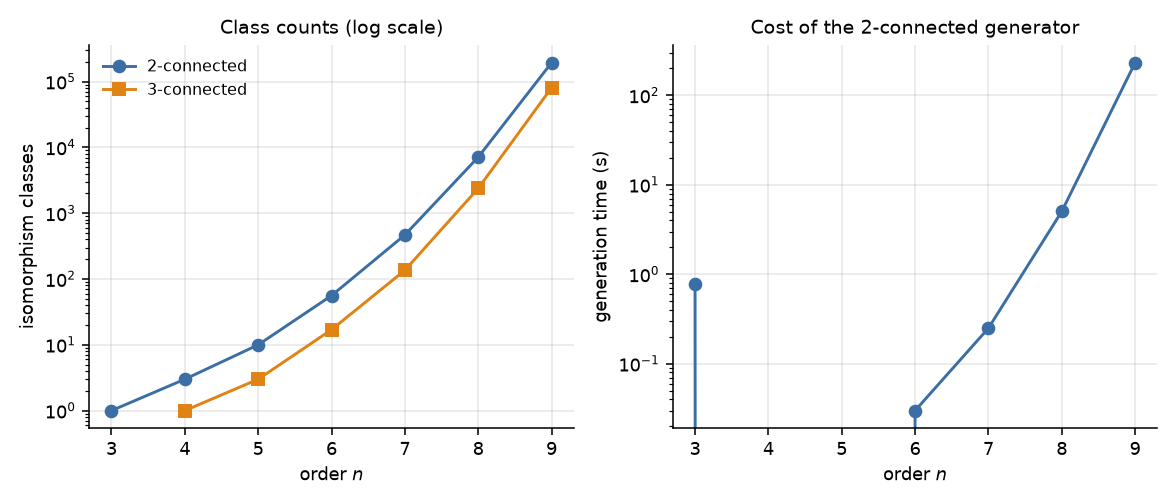
\includegraphics[width=0.82\textwidth]{../figures/fig_growth.png}
\caption{Left: growth of the enumerated class counts (logarithmic scale).
Right: measured cost of the $2$-connected generator.}
\label{fig:growth}
\end{figure}

\section{Limitations and open problems}\label{sec:limitations}

We are explicit about what this paper does not establish.

\begin{description}[leftmargin=0pt,style=nextline]
\item[Conjecture~\ref{conj:sharp} is open.]  We verify it exhaustively for
  $n\le 9$, and it holds for graphs with a dominating vertex
  (Corollary~\ref{cor:wheel}), but a cubic $3$-connected graph of order $20$ is
  out of reach of the bounds proved here: \eqref{eq:combo} gives only
  $c(G)\ge c(K_4)=7$ and $c(G)\ge 3|E|-3n+1=2n-1$.  A proof needs a genuinely
  new way of trading the number of long paths against the number of long
  cycles.  We also note that Conjecture~\ref{conj:sharp} is loose on the
  computed range: $m_3(n)/\binom{n-1}{2}$ takes the values
  $7/3,\,13/6,\,14/10,\,24/15,\,26/21,\,42/28$ for $n=4,\dots,9$.
\item[Conjecture 6(a) of \cite{mcculloch2026} is not settled.]  Our computation
  agrees with it below $51$, but ruling out a cycle count $m$ for all $n$
  requires an order bound in terms of $m$ that is (i) valid for all
  $3$-connected graphs and (ii) small enough to be enumerable.
  Theorem~\ref{thm:decid} gives $|V(G)|\le 2(m-1)$, far too weak, while
  Conjecture~\ref{conj:sharp} would give $|V(G)|\le 9$ for $m\le 34$ --- exactly
  the range we enumerate.  There is therefore a clean logical dependency: the
  low part of the $3$-connected spectrum is conjecturally one finite
  computation away.
\item[$m_3(n)$ is known only for $n\le 9$.]  Our generators produce all
  $3$-connected graphs of order at most $9$ ($80890$ classes); $m_3(10)$ is
  not reported rather than guessed.
\item[The spectra $S_k$ for $k\ge 4$ are only sampled.]  On orders at most $7$
  we find $|S_4|=30$ and $|S_5|=5$; Theorem~\ref{thm:A} supplies the exact
  minima $c(K_5)=37$ and $c(K_6)=197$ for those classes, but the exception sets
  of $S_4$ are undetermined.
\item[Equality in Lemma~\ref{lem:path} for $r=2$.]  The bound
  $p_F(x,y)\ge Q_3=2$ is sharp, but equality is achieved by every $2$-connected
  graph in which $x$ and $y$ are joined by exactly two paths, a large and
  structurally unclassified class containing all cycles.  Theorem~\ref{thm:A}
  avoids this case by using $\delta(G)\ge 3$ in the inductive step.
\item[No claim about the existence direction of Conjecture 6(a).]  Showing
  that every $m\ge 35$ is the cycle count of some $3$-connected graph is a
  construction problem that we did not attack; our computation only certifies
  existence for $m\le 34$.
\end{description}

Two directions seem promising.  First, $m_3(n)$ appears to be attained by
graphs that are as regular as their order allows --- every minimiser we found is
$3$-regular when $3n$ is even, and otherwise has the most balanced degree
sequence permitted by parity --- and proving that heuristic would turn
Table~\ref{tab:m3} from a computation into a theorem.  Second,
Theorem~\ref{thm:A} says nothing about graphs of prescribed order; a sharp
order-sensitive bound is exactly what Conjecture~\ref{conj:sharp} asks for, and
its failure to follow from the path-counting machinery suggests that the right
object is not the number of paths but the number of cycles through a fixed
vertex, where the extremal configuration is a cone.

\section{Conclusion}

Two clean statements organise the cycle content of highly connected graphs:
among cones, wheels are extremal, and complete graphs are the sparsest
$k$-connected graphs of their class (Theorems~A and~B); and the spectra
$S_k$ are computable with an explicit order reduction (Theorem~C).
Computationally we obtain $m_3(n)$ for $4\le n\le 9$ and reproduce the
conjectured exception set of $S_3$ below $51$.  The open core is
Conjecture~\ref{conj:sharp}, the order-sensitive version of Theorem~A, which
we have identified as the single missing ingredient for turning the low part of
the $3$-connected spectrum into a finite computation.

\begin{thebibliography}{99}
\small
\bibitem{mcculloch2026}
R.~McCulloch, B.~D. McKay, A.~Salahshoori and T.~Zaslavsky.
\newblock The cycle counts of graphs.
\newblock \emph{Graphs and Combinatorics} 42 (2026), 53--.
\newblock Preprint arXiv:2507.02260.

\bibitem{whitney1932}
H.~Whitney.
\newblock Non-separable and planar graphs.
\newblock \emph{Trans. Amer. Math. Soc.} 34 (1932), 339--362.

\bibitem{aldred1997cycles}
R.~E.~L. Aldred and C.~Thomassen.
\newblock On the number of cycles in $3$-connected cubic graphs.
\newblock \emph{J. Combin. Theory Ser. B} 71 (1997), 79--84.

\bibitem{carmesin2025}
J.~Carmesin and J.~Kurkofka.
\newblock Canonical decompositions of $3$-connected graphs.
\newblock \emph{Advances in Combinatorics} 2025:7, 1--73.

\bibitem{czabarka2009}
\'E.~Czabarka, L.~Sz\'ekely and S.~Wagner.
\newblock The inverse problem for certain tree parameters.
\newblock \emph{Discrete Appl. Math.} 157 (2009), 3314--3319.

\bibitem{mckay2014practical}
B.~D. McKay and A.~Piperno.
\newblock Practical graph isomorphism, II.
\newblock \emph{J. Symbolic Comput.} 60 (2014), 94--112.

\bibitem{brinkmann2011cubic}
G.~Brinkmann, J.~Goedgebeur and B.~D. McKay.
\newblock Generation of cubic graphs.
\newblock \emph{Discrete Math. Theor. Comput. Sci.} 13 (2011), 69--80.

\bibitem{read1956number}
R.~C. Read.
\newblock The number of graphs with various properties.
\newblock \emph{Trans. Amer. Math. Soc.} 84 (1956), 118--134.

\bibitem{harary1973graphical}
F.~Harary and E.~M. Palmer.
\newblock \emph{Graphical Enumeration}.
\newblock Academic Press, 1973.

\bibitem{volkmann1996}
L.~Volkmann.
\newblock Estimations for the number of cycles in a graph.
\newblock \emph{Periodica Mathematica Hungarica} 33 (1996), 153--161.

\bibitem{dvorak2021}
Z.~Dvo\v{r}\'ak.
\newblock Bounding the number of cycles in a graph in terms of its degree
  sequence.
\newblock \emph{J. Combin. Theory Ser. B} (2021).
\newblock \url{https://www.sciencedirect.com/science/article/pii/S019566982030127X}.

\bibitem{locke1982}
S.~C. Locke.
\newblock Relative lengths of paths and cycles in $k$-connected graphs.
\newblock \emph{J. Combin. Theory Ser. B} (1982).
\newblock \url{https://www.sciencedirect.com/science/article/pii/0095895682900363}.

\bibitem{diestel2017}
R.~Diestel.
\newblock \emph{Graph Theory}, 5th edition.
\newblock Springer, 2017.

\bibitem{oeisA002807}
The OEIS Foundation Inc.
\newblock A002807: number of cycles in the complete graph on $n$ nodes.
\newblock \url{https://oeis.org/A002807}.

\bibitem{oeisA385523}
The OEIS Foundation Inc.
\newblock A385523: numbers that are not cycle counts of inseparable graphs.
\newblock \url{https://oeis.org/A385523}.

\bibitem{igraph}
igraph: Python interface to the igraph library.
\newblock \url{https://python.igraph.org}.
\end{thebibliography}

\appendix

\section{Identities}\label{app:identities}

\subsection{The cycles of a complete graph}
A cycle of length $j$ in $K_n$ is a $j$-element vertex set together with one
of $(j-1)!/2$ cyclic orders, so
\[
  c(K_n)=\frac12\sum_{j=3}^{n}\binom nj (j-1)! ,
\]
giving $1,7,37,197,1172,8018,62814$ for $n=3,\dots,9$, in agreement with
\cite{oeisA002807} and with the values computed independently by our code.

\subsection{The recurrence for $Q_k$}
Recall $Q_m=\sum_{j=0}^{m-2}\binom{m-2}{j}j!$.  Since
$\binom{m-2}{j}j! = (m-2)!/(m-2-j)!$, putting
$E_t=\sum_{i=0}^{t}1/i!$ and substituting $i=m-2-j$ gives
$Q_m=(m-2)!\,E_{m-2}$, whence for $r\ge2$
\[
  Q_{r+1}=(r-1)!E_{r-1}
         =(r-1)!\Big(E_{r-2}+\tfrac{1}{(r-1)!}\Big)
         =(r-1)\,(r-2)!\,E_{r-2}+1
         =(r-1)Q_r+1 ,
\]
and $Q_2=0!\,E_0=1$.  This proves Lemma~\ref{lem:rec}.

\subsection{Why $\cF=1$ forces $F$ to be a cycle}
If $c(F)=1$ and some vertex $x$ has degree $d\ge 3$, pick distinct
neighbours $y,z$ of $x$.  In a $2$-connected graph there is a $y$-$z$ path
avoiding $x$ (otherwise $x$ is a cut vertex), so $x\,y P z\,x$ is a second
cycle, a contradiction.  Hence $\delta(F)=2$ whenever $c(F)=1$, and a
$2$-regular graph is a disjoint union of cycles, of which only one may be
present since $c(F)=1$.  Symmetrically, $c(K_1\vee F)=1$ is impossible for
$|V(F)|\ge 3$.

\section{What the accompanying code checks}

\begin{itemize}[leftmargin=*]
\item $c$ and $p(x,y)$ agree with \texttt{networkx} on all graphs with at most
  five vertices, and with an independent brute-force search over $2$-regular
  connected edge subsets on all graphs with at most five vertices; the
  $n=6$ case is checked by brute force as well.
\item $\kappa$ agrees with \texttt{networkx} on all graphs with at most six
  vertices.
\item The generators agree with exhaustive brute force, as \emph{sets of
  canonical labels}, for both connectivity classes and $n\le 6$ inside the test
  suite, and for $n\le 7$ via \texttt{scripts/validate\_generators.py}.
\item Lemma~\ref{lem:path} holds on all pairs of vertices of all
  $2$-connected graphs with $n\le 7$, with its equality condition checked
  exhaustively for $r\ge 3$ and a recorded counterexample to the naive
  statement at $r=2$.
\item Theorem~\ref{thm:A} and Corollary~\ref{cor:wheel} hold on all
  $3$-connected graphs with $n\le 9$.
\item Conjecture~\ref{conj:sharp} holds on all $3$-connected graphs with
  $n\le 7$.
\item The spectrum statements of Section~\ref{sec:comp}(ii) are regression
  tested.
\end{itemize}

\end{document}